\documentclass{article}
\usepackage[utf8]{vietnam}
\usepackage[14pt]{extsizes}
\usepackage{amsmath,amsfonts,amsthm}
\usepackage{geometry}
\usepackage{graphicx}
 \geometry{
 a4paper,
 total={170mm,257mm},
 left=20mm,
 top=20mm,
}
\usepackage{enumitem} 
\title{Đề kiểm tra 2}
\begin{document}
\maketitle
\textit{Lưu ý: Thời gian làm bài chỉ có \textbf{60 phút} và \textbf{không} được sử dụng máy tính Casio hay bất cứ tài liệu nào.}
\begin{enumerate}[start=1,label={\bfseries Câu  \arabic*:},leftmargin=1in]
    \item Cho hàm số $f(x)$ được xác định như sau:
    $$f(x)=\frac{x-2}{\sqrt{|x^2-3|-6}}+\sqrt{9-x^2}$$
\begin{enumerate}
    \item Tìm tập xác định của hàm số $f(x)$.
    \item Hàm số $f(x)$ có tồn tại không? Vì sao?
\end{enumerate}
    \item Giải hệ phương trình sau:
    \begin{equation*}
        \left\{\begin{aligned}
            &&x^3+xy^2-yx^2-y^3=0\\
            &&\sqrt{y^2-4}+|x-2|=0\\
        \end{aligned}\right.
    \end{equation*}
    \item Một dòng nước đang chảy qua một ống cao su như hình vẽ:
    \begin{figure}[h]
        \centering
        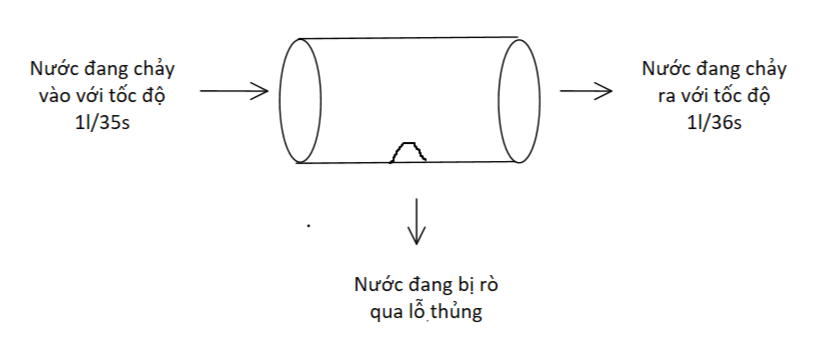
\includegraphics[width=0.9\textwidth]{a_pipe.png}
        \label{nem_ngang}
        \end{figure}
   \\Sau bao lâu thì $1l$ nước bị rò qua lỗ thủng?
   \item Cho tam giác $\triangle ABC$ vuông tại $A$ có đường cao $AH$ vuông góc với đáy $BC$. Hãy chứng minh hệ thức sau:
   $$\frac{1}{AH^2}=\frac{1}{AB^2}+\frac{1}{AC^2}$$
\end{enumerate}
\end{document}